\documentclass[a4paper,11pt]{article}
    \usepackage{titling}
    \usepackage[left=2cm, right=2cm, top=2cm]{geometry}
    \usepackage{mathtools}
    \usepackage{graphicx}
    \usepackage{float}
    \title{\vspace{-2.0cm}EMP191 Rocket Lab 9}
    \author{Warren Yuan}
    \date{\today}
    
    
    \begin{document}
    
    \maketitle
    
    \begin{abstract}
     {In this lab, students used Mathematica to make a model of and plot the trajectory of the rocket launch, based on differential equations to model the air leaving the bottle in between two phases.}
    \end{abstract}
    
    \section{Introduction}
    {\quad The goal of this lab was to be able to make an accurate model of the trajectory using Newton's laws, as well as become more well versed in Mathematica and trajectory modelling.}
    
    \section{Measurement Procedure}
    {\quad The procedure was followed through as written.}
    
    % \section{Plots of Data}
    % \begin{figure}[H]
    %     \begin{center}
    %     %\includegraphics[width=\linewidth/3]{}
    %     \end{center}
    %     \caption{Using acceleration minimum to adjust position}
    %     \label{fig:Rocket Trajectory}
    % \end{figure}
    % \begin{figure}[H]
    %     \begin{center}
    %     %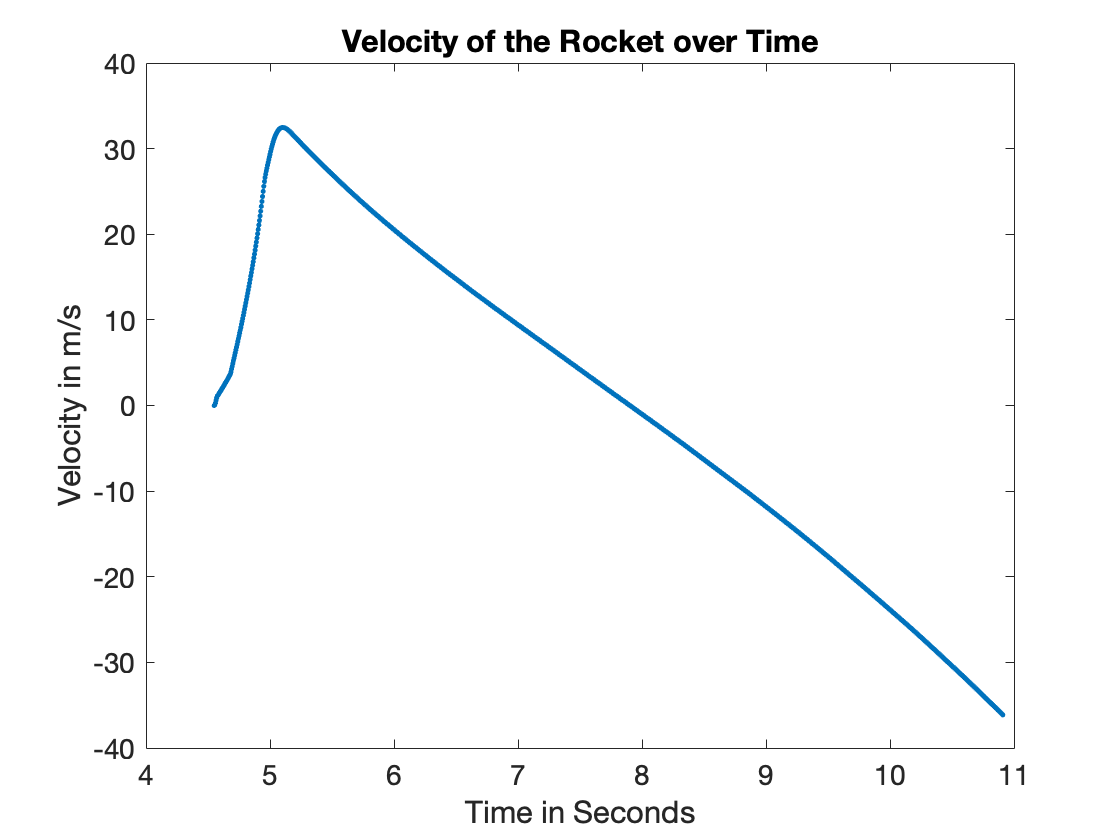
\includegraphics[width=\linewidth/3]{vel.png}
    %     \end{center}
    %     \caption{Graph of Velocity}
    %     \label{fig:Velocity}
    % \end{figure}
    % \begin{figure}[H]
    % \begin{center}
    %     %`  1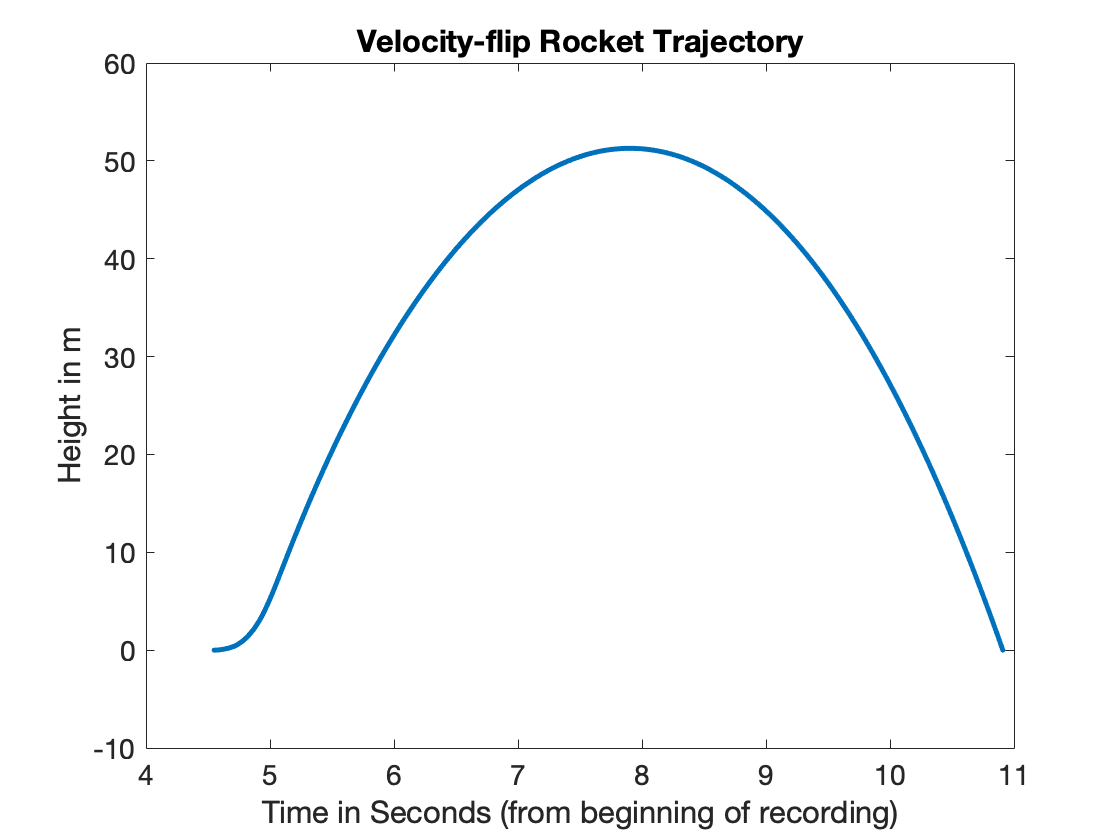
\includegraphics[width=\linewidth/3]{velrkttraj.png}
    % \end{center}
    %     \caption{Using Velocity sign-flip to adjust position}
    %     \label{fig:Rocket Trajectory}
    % \end{figure}
    
    \section{Analysis Results}
    {}
    {For part A, we began with the equation: }
    \begin{equation} 
       p_{10} = p_{0}(V_{0}/V(t))^{\gamma} = 4.4*10^5*\frac{.0015}{.002}^{\frac{7}{5}} = 294129.4056
    \end{equation}
    {}
    \begin{equation}   
        \frac{d\rho_{1}}{dt} = -\frac{dm}{dt} * \frac{1}{V(t)}
    \end{equation}
    \begin{equation}   
        \Delta x = v0 + at^2 \rightarrow \quad 0.22 = 0 + 155t^2 \rightarrow \quad t = 0.0377s
    \end{equation}
    {Part B: Using Bernoulli's Equation}
    \begin{equation} 
        P_{1} + \rho gh_{1} + \frac{1}{2}\rho v_{1}^2 = P_{2} + \rho gh_{2} + \frac{1}{2}\rho v_{2}^2\rightarrow\quad  P_{1} = P_{2} + \frac{1}{2}\rho v_{2}^2\rightarrow \quad v_{2} = \sqrt{\frac{2(P_{1} - P_{2})}{\rho}}  
    \end{equation}
    {where $v_{2}$ is the exit velocity of the water from the rocket and $A_{n}$ is the area of the bottle nozzle.}
    \begin{equation}
        v_{2} = \sqrt{\frac{2(4.40*10^5- 10^5)}{1000}} = 26.07m/s
    \end{equation}
    {here is the derivation of $\frac{dM}{dt}$ for 0.27 seconds until depletion.}
    \begin{equation}
        \frac{dM}{dt} = Area * v_{2} * 1000 = 1.84 kg/s  
    \end{equation}
    {Using the Rocket Equation and Newton's laws one can derive the differential equation for $\frac{dv}{dt}$.}
    \begin{equation}
        \frac{dv}{dt} = -u*ln(\frac{M_{i}-\frac{dM}{dt}t}{M_{i}}) - gt
    \end{equation}
    {The drag force equation is derived below: where $A_{b}$ is the area of the bottle cross section and $m_{e}$ is the mass of the empty rocket.}
    \begin{equation}
        mg \pm kv^2 = ma \rightarrow \quad g \pm \frac{kv^2}{m_{e}} = \frac{dv}{dt} \rightarrow \quad 
        \frac{dv}{dt} = g \pm \frac{\rho_{a} A_{b}C_{d}v^2}{2m_{e}}
    \end{equation}
    
    \begin{figure}[H]
        %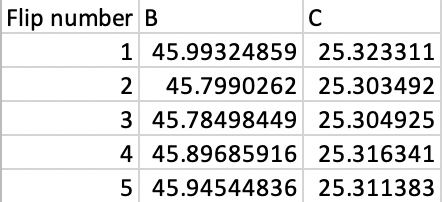
\includegraphics[width=\linewidth/4]{table.png}
    \end{figure}
    
    {}
    
    {For Launch Tube Time : Solving for time with the equation above (and acceleration = $155m/s^2$) we get 0.0377s which is relatively close to my time of 0.0234s obtained in the previous lab. I used the times from the previous lab for the phases 2-4, getting t2 = 5.175, t3 = 7.9 seconds}
    
    \section{Conclusion}
    {The improved model took into account the friction of the tube as well as the air resistance causing drag. The use of the angles helped to correct the trajectory.}
    \end{document}
    
    